\subsection{Упражнение 1}

Пилообразный сигнал линейно нарастает от -1 до 1, а затем резко падает до -1 и повторяется.

\noindent Напишите класс, называемый SawtoothSignal, расширяющий signal и предоставляющий evaluate для оценки пилообразного сигнала.

\noindent Вычислите спектр пилообразного сигнала. Как соотносится его гармоническая структура с тругольными с прямоугольными сигналами?

Для создания пилообразного сигнала создадим класс SawtoothSignal. В методе класса evaluate опишем число циклов и c помощью библиотеки numpy разделим число циклов. unbias - смещает сигнал а normalize масштабирует его до заданной амплитуды.

\begin{lstlisting}[language=Python]
import thinkdsp

class SawtoothSignal(thinkdsp.Sinusoid):
  def evaluate(self, ts):
    cycles = self.freq * ts + self.offset / np.pi / 2
    frac, _ = np.modf(cycles)
    ys = thinkdsp.normalize(thinkdsp.unbias(frac), self.amp)
    return ys
\end{lstlisting}

\noindent Отобразим график пилообразного сигнала.

\begin{lstlisting}[language=Python]
saw = SawtoothSignal()
saw.plot()
saw_wave = saw.make_wave(duration=3, framerate=10000)
\end{lstlisting}

\begin{figure}[H]
	\begin{center}
		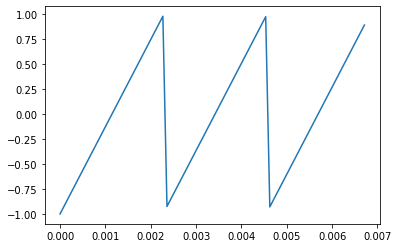
\includegraphics[scale=1]{fig/lab02/lab02_1.png}
		\caption{График пилообразного сигнала}
	\end{center}
\end{figure}

Вычислим спектр.

\begin{lstlisting}[language=Python]
spectr = saw_wave.make_spectrum()
spectr.plot()
\end{lstlisting}

\begin{figure}[H]
	\begin{center}
		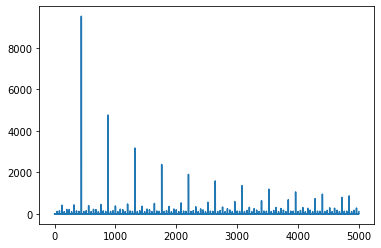
\includegraphics[scale=1]{fig/lab02/lab02_2.png}
		\caption{Спектр пилообразного сигнала}
	\end{center}
\end{figure}

Теперь сравним полученный спектр с треугольными и прямоугольными сигналами.

\begin{lstlisting}[language=Python]
triangle = TriangleSignal()
triangle.make_wave(duration=3, framerate=10000).make_spectrum().plot()
\end{lstlisting}

\begin{figure}[H]
	\begin{center}
		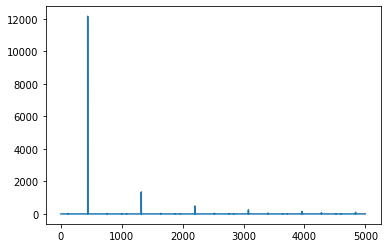
\includegraphics[scale=1]{fig/lab02/lab02_3.png}
		\caption{Спектр треугольного сигнала}
	\end{center}
\end{figure}

\begin{lstlisting}[language=Python]
square = SquareSignal()
square.make_wave(duration=3, framerate=10000).make_spectrum().plot()
\end{lstlisting}

\begin{figure}[H]
	\begin{center}
		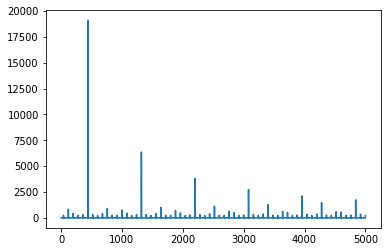
\includegraphics[scale=1]{fig/lab02/lab02_4.png}
		\caption{Спектр прямоугольного сигнала}
	\end{center}
\end{figure}

Можно заметить, в сравнении с треугольным сигналом, его амплитуда падает пропорцианально квадрату частоты, а у пилообразного пропорцианально частоте, ровно также как и у квадратного сигнала, однако пилообразный включает в себя как четные, так и нечетные гармоники, когда у квадратного только нечетные.

\subsection{Упражнение 2}

Создайте прямугольный сигнал 1100 Гц и вычислите wave с выборками 10 000 кадров в секунду. Постройте спектр и убедитесь, что большинство гармоник "завёрнуты" из-за биений, слышно ли последствия этого при проигрывании?

\begin{lstlisting}[language=Python]
square = thinkdsp.SquareSignal(1100)
segment = square.make_wave(duration=1, framerate=10000)
spectr = segment.make_spectrum()
spectr.plot()
\end{lstlisting}

\begin{figure}[H]
	\begin{center}
		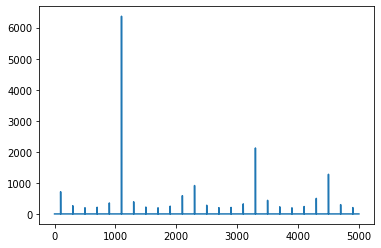
\includegraphics[scale=1]{fig/lab02/lab02_5.png}
		\caption{Спектр сигнала с биениями}
	\end{center}
\end{figure}

На спектре видно, что происходит "завернутость" биений, гармоники 1100 и 3300 выстроены верно, однако видно, что третий и четвертый пик находятся на 4500 и 2300 соответственно, они неотличимы от 5500 и 7700


\subsection{Упражнение 3}

Возьмите объект спектра spectrum, и выведите первые несколько значений spectrum.fs, вы увидите, что частоты начинаются с нуля. Итак, «spectrum.hs[0]» — это величина компонента с частотой 0. Но что это значит?

\noindent Попробуйте этот эксперимент:

1. Сделать треугольный сигнал с частотой 440 и создать Волну длительностью 0,01 секунды. Постройте форму волны.

2. Создайте объект Spectrum и напечатайте spectrum.hs[0]. Каковы амплитуда и фаза этой составляющей?

3. Установите spectrum.hs[0] = 100. Создайте волну из модифицированного спектра и выведите ее. Как эта операция влияет на форму сигнала?

Создадим треугольный сигнал с частотой 440Hz и длительностью 0,01 сек, построим его график, распечатаем сигнал и распечатаем Spectrum.hs[0].


\begin{lstlisting}[language=Python]
signal = thinkdsp.TriangleSignal(440)
segment = signal.make_wave(0.01, framerate=10000)
segment.plot()
\end{lstlisting}

\begin{figure}[H]
	\begin{center}
		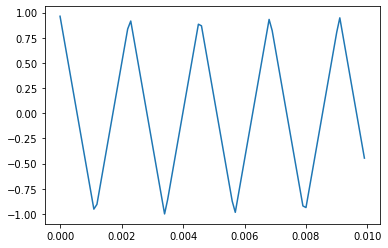
\includegraphics[scale=1]{fig/lab02/lab02_6.png}
		\caption{График сигнала}
	\end{center}
\end{figure}

Проверим что лежит в 0 элементе.

\begin{lstlisting}[language=Python]
spectr = segment.make_spectrum()
spectr.hs[0]
\end{lstlisting}

\begin{lstlisting}
(3.375077994860476e-14+0j)
\end{lstlisting}
Каждый элмент массива hs объекта Spectrum представялет собой комплексное число. Они соотвествуют частотной компоненте: размах пропоцианален амплитуде соответствующей компоненты, а угол - это фаза.

\noindent Видно, что первый элемент массива hs - это комплексное число близкое к нулю. Установим этому элементу значение 100 и посмотрим на результат
\begin{lstlisting}[language=Python]
spectr.hs[0] = 100
spectr.make_wave().plot()
\end{lstlisting}

\begin{figure}[H]
	\begin{center}
		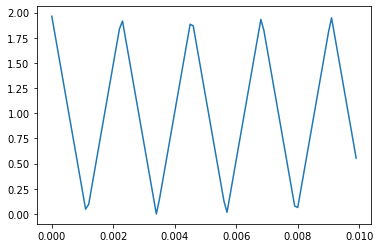
\includegraphics[scale=1]{fig/lab02/lab02_7.png}
		\caption{График сигнала с изменённым нулевым числом спекторграммы}
	\end{center}
\end{figure}

Из полученного графика видно смещение сигнала по вертикали, таким образом можно сделать вывод о том, что первый элемент отвечает за смещение по вертикали, в случае, если он близок к нулю, то сигнал не смещается.

\subsection{Упражнение 4}

Напишите функцию, которая принимает Spectrum в качестве параметра и модифицирует его, деля каждый элемент hs на соответствующую частоту из fs. Протестируйте свою функцию, используя один из файлов WAV в репозитории или любой объект Wave.

1. Рассчитайте спектр и начертите его.

2. Измените спектр, используя свою функцию, и снова начертите его.

3. Сделать волну из модифицированного Spectrum и прослушать ее. Как эта операция влияет на сигнал?


Напишем функцию которая принимает на вход Spectrum и изменяет его его делением каждого элемента hs на соответствующую частоту fs и проверим эту функцию на треугольном сигнале

\begin{lstlisting}[language=Python]
def spec_div(spec):
  spec.hs[1:] /= spec.fs[1:]
  spec.hs[0] = 0
  spec.plot()

triangle = TriangleSignal()
wave = triangle.make_wave(duration=0.5, framerate=10000)
wave.make_audio()

spectr = wave.make_spectrum()
spectr.plot()
\end{lstlisting}

\begin{figure}[H]
	\begin{center}
		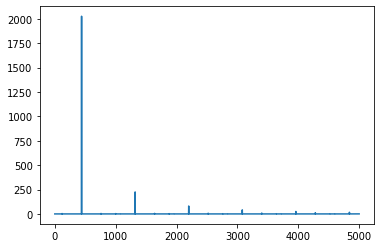
\includegraphics[scale=1]{fig/lab02/lab02_8.png}
		\caption{Спектр треугольного сигнала}
	\end{center}
\end{figure}

Применим написанную функцию.

\begin{lstlisting}[language=Python]
spec_div(spectr)
\end{lstlisting}

\begin{figure}[H]
	\begin{center}
		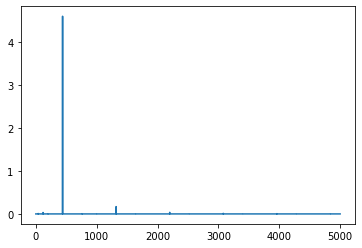
\includegraphics[scale=1]{fig/lab02/lab02_9.png}
		\caption{Спектр изменённого сигнала}
	\end{center}
\end{figure}

\begin{lstlisting}[language=Python]
spectr.make_wave().make_audio()
\end{lstlisting}

Если прослушать полученный звук, можно услышать что он стал тише и чище, это связано с работой функции, которая ослабляет низкие частоты на некоторую величину.

\subsection{Упражнение 5}

Треугольные и прямоугольные волны имеют только нечетные гармоники; пилообразная волна имеет как четные, так и нечетные гармоники. Гармоники прямоугольной и пилообразной волн затухают пропорционально $1/f$; гармоники треугольной волны затухают как $1/f^2$. Можете ли вы найти форму волны, в которой четные и нечетные гармоники затухают как $1/f^2$?

\noindent Подсказка: есть два способа подойти к этому: вы можете построить нужный сигнал путем сложения синусоид, или вы может начаться с сигнала, похожего на то, что вы хотите, и изменить его.


\noindent Создадим сигнал, состоящий из четных и нечетных гармоник, при этом, чтобы они падали пропорцианально квадрату частоты. Возьмем пилообразный сигнал, который имет четные и нечетные гармоники, а далее скорректируем его спад при помощи функции из предыдущего упражнения.

\begin{lstlisting}[language=Python]
saw_sign = SawtoothSignal(400)
saw_w = saw_sign.make_wave(duration=0.5, framerate=20000)
spectr = saw_w.make_spectrum()
spectr.plot()
decorate(xlabel='Frequency (Hz)')
\end{lstlisting}

\begin{figure}[H]
	\begin{center}
		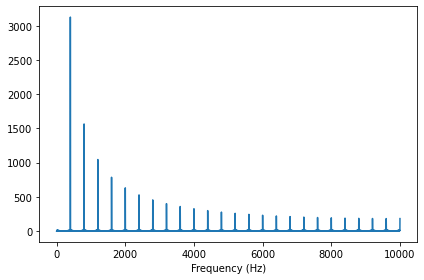
\includegraphics[scale=1]{fig/lab02/lab02_10.png}
		\caption{Спектр пилообразного сигнала}
	\end{center}
\end{figure}

Применим функцию для изменения амплитуды спада

\begin{lstlisting}[language=Python]
spec_div(spectr)
spectr.scale(400)
spectr.plot()
\end{lstlisting}

\begin{figure}[H]
	\begin{center}
		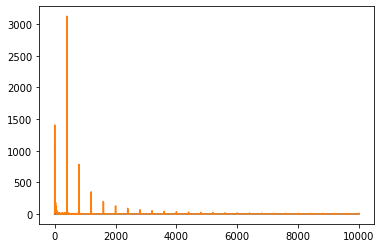
\includegraphics[scale=1]{fig/lab02/lab02_11.png}
		\caption{Спектр пилообразного сигнала после функции}
	\end{center}
\end{figure}

\begin{lstlisting}[language=Python]
spectr.make_wave().segment(duration=0.01).plot()
\end{lstlisting}

\begin{figure}[H]
	\begin{center}
		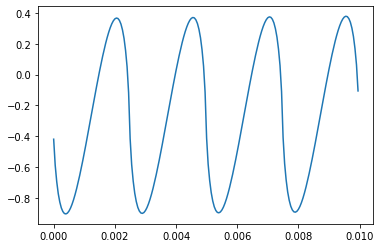
\includegraphics[scale=1]{fig/lab02/lab02_12.png}
		\caption{График сигнала}
	\end{center}
\end{figure}

Видно, что спектр спадает пропорционально квадрату частоты и при этом имеет четные и нечетные гармоники

\subsection{Вывод}

В данной работе были произведены различные действия с разными видами сигналов, были рассмотрены спектры и гармонические структуры и биения.